\section{Auswertung}
\label{sec:Auswertung}
\subsection{Bestimmung der Apparatekonstante \texorpdfstring{$K_{gr}$}{math}}
\label{sec:BdA}
Zuerst wird mit der Gleichung
\begin{equation}
  \eta = K (\rho_k - \rho_{Fl})t
  \label{eqn:eta1}
\end{equation}
die Viskosität $\nu$ ermittelt. Dabei beschreibt $\rho_k$ die Dichte der Kugel,
$\rho_{Fl}$ die Dichte der Flüssigkeit, $K$ die Apparatekonstante abhängig von
der Kugel und $t$ die Fallzeit.
Die Apparatekonstante ist für die kleine Kugel mit $K_{kl} = 7,64 \cdot 10^{-5}
\,\si{\milli\pascal\meter\tothe{3}\per\kilo\gram} $
gegeben. Im Folgenden wird die Dichte $\rho_{Fl}$ des destillierten Wassers, mit
1000 \si{\kilo\gram\per\meter\tothe{3}} angenommen. Mit der Gleichung
\begin{equation*}
  \rho_{k} = \frac{m}{\frac{4}{3}\pi\left(\frac{d}{2}\right)^3}
\end{equation*}
lässt sich die Dichte der beiden Kugeln bestimmen. Dabei bezeichnet $m$ das
Gewicht der Kugel und $d$ den Durchmesser der Kugel. Das Gewicht der Kugeln
beträgt 4,45 \si{\gram} für die kleine Kugel und 4,95 \si{\gram} für die große
Kugel. Für $d$ wird das Mittel aus den gemessenen Durchmesser genommen. Dann
ergibt sich für den Durchmesser der kleinen Kugel ca. (0,01558 \si{\meter} und
für die große Kugel ca. 0,01575 \si{\meter}.
Daraus ergibt sich dann für die Dichte der kleinen Kugel $\rho_{kl} =
(2243.8 \pm 0.9) \si{\kilo\gram\per\meter\tothe{3}}$ und für die große Kugel
$\rho_{gr} = (2415.7 \pm 0.6) \si{\kilo\gram\per\meter\tothe{3}} $.
Schlussendlich ergibt sich dann
für die Viskosität, brechnet anhand der Daten der kleinen Kugel,
$(1.2084 \pm 0.0032)\si{\milli\pascal\second}$.
Aus der Gleichung \eqref{eqn:eta1} folgt nun die Beziehung
\begin{equation*}
  K_{gr} = \frac{\eta}{(\rho_{gr} - \rho_{Fl})t_{gr}}
        = \frac{K_{kl} (\rho_{kl} - \rho_{Fl})t_{kl}}{(\rho_{gr} - \rho_{Fl})t_{gr}}\, ,
\end{equation*}
dabei bezeichnet $t_{kl}$ das Mittel der Fallzeit der kleinen Kugel und $t_{gr}$
das Mittel der Fallzeit der großen Kugel. Der Wert für $t_{kl}$ liegt bei
$(12.71 \pm 0.033) \si{\second}$ und für $t_{gr}$ bei $(85.84 \pm 0.22)
\si{\second}$. Daraus ergibt sich die Apparatekonstante $K_{gr}  = (9.94 \pm 0.04)
\cdot 10^{-6} \si{\milli\pascal\meter\tothe{3}\per\kilo\gram}$.
\subsection{Temperaturabhängigkeit der Viskosität}
Zuerst wird mit der Gleichung \eqref{eqn:eta1} die Viskosität brechnet, logarithmiert
und gegen $\frac{1}{T}$ aufgetragen, hierbei ist $T$ natürlich die Temperatur.
Wird nun eine Ausgleichrechnung mit
\begin{equation*}
  \symup{ln}(\eta)= \frac{B}{T}\cdot\symup{ln}(A)
\end{equation*}
durchgeführt, so ergibt sich die Konstante $ A =  (0.00297 \pm 0.00022)
\si{\milli\pascal\second}$ und $B = (1756 \pm 23) \si{\kelvin}$. Der soeben
beschriebene Vorgang ist in Abbildung \ref{fig:plot} dargestellt.
\begin{figure}
  \centering
  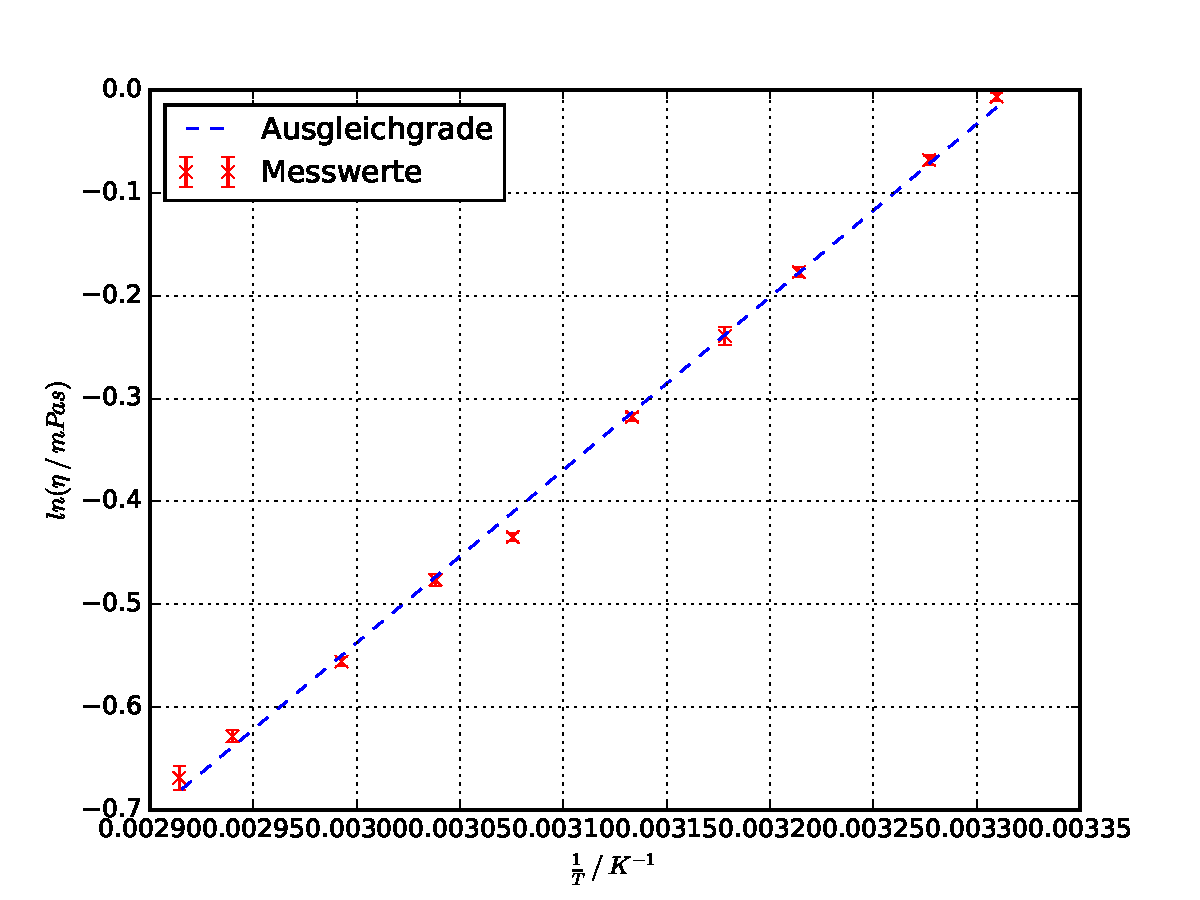
\includegraphics[height= 7cm]{Plots/plot.pdf}
  \caption{Temperaturabhängigkeit der Viskosität}
  \label{fig:plot}
\end{figure}
Die oben genannte Gleichung zur Ausgleichsrechnung kommt von der Andratschen
Gleichung \cite{Anleitung}, diese Beschreibt die Temperaturabhängigkeit der
Viskosität wie folgt:
\begin{equation*}
  \eta(T) = A\cdot \symup{exp}\left(\frac{B}{T}\right)\,.
\end{equation*}
Werden die Konstanten in die Gleichung eingesetzt ergibt sich für die Viskosität
im Mittel $(0.856 \pm 0.032) \si{\milli\pascal\second}$. Dabei ist zu beachten,
dass das destillierte Wasser seine Dichte mit der Temperatur ändert. Deshalb
werden nur Werte in die Ausgleichsrechnung, sowie in der Brechnung der
Viskosität einbezogen, die den Signifikanzbereich nicht verletzen.
\subsection{Reynolds-Zahl}
Die Reynolds-Zahl \cite{wiki} ist definiert durch
\begin{equation*}
  Re = \frac{\rho\cdot v\cdot d}{\eta}.
\end{equation*}
Dabei bezeichnet $\rho$ die Dichte des Mediums $v$ die Strömungsgeschwindigkeit,
$d$ der Durchmesser des Rohrs und $\eta$ die Viskosität.
Da das destillierte Wasser nicht
strömt, wird hier die Fallgeschwindigkeit der Kugel benutzt.
Für die Werte aus Kapitel \ref{sec:BdA} ergibt sich
für die kleine Kugel $Re = (50.72 \pm 0.26)$ und für die große Kugel
$ Re = (7.596 \pm 0.026) $. Da diese Zahlen wesentlich kleiner sind als
1150 kann von einer laminaren Strömung ausgegangen werden.




























%
